\documentclass{beamer}

% Thème personnalisé
\usetheme{lines}

% Quelques importations pratiques
\usepackage{ifthen}      % pour des confitions dans les commandes
\usepackage{multicol}    % environnement multi colonnes
\usepackage{booktabs}    % pour des tables propres et sans colonnes
\usepackage{pifont}      % des symboles en plus
\usepackage{fontawesome} % utilisation de police d'icônes web
\usepackage{listings}
\usepackage{color}
%% Font recommendations
%\usepackage{fontspec}
%\usepackage[math]{kurier} % main font
%\usepackage[T1]{fontenc} % font encoding
%\DeclareTextCommandDefault{\nobreakspace}{\leavevmode\nobreak\ } % Because T1 disable this command, we redefine it
%\usepackage{fontawesome} % to have web fonts


\usepackage{fontspec}
\usepackage[math]{kurier} % main font
%\usepackage[T1]{fontenc} % font encoding
\DeclareTextCommandDefault{\nobreakspace}{\leavevmode\nobreak\ } % Because T1 disable this command, we redefine it
\newfontfamily\aniron{Aniron}
\newfontfamily\titlePageFont{Canter Bold}
\setmainfont{Fira Sans Light}

%%% Local Variables:
%%% mode: latex
%%% TeX-master: "../XGBoost"
%%% End:

\definecolor{codegreen}{rgb}{0,0.6,0}
\definecolor{codegray}{rgb}{0.5,0.5,0.5}
\definecolor{codepurple}{rgb}{0.58,0,0.82}
\definecolor{backcolour}{rgb}{0.95,0.95,0.92}

% Define Language
\lstdefinelanguage{minizinc}
{
  % list of keywords
  morekeywords={ann,annotation,any,assert,bool,constraint,enum,float,function,in,include,int,list,of,op,output,minimize,maximize,par,predicate,record,set,solve,string,test,tuple,type,var,where},%
  emph={abort,abs,acos,acosh,array_intersect,array_union,array1d,array2d,array3d,array4d,array5d,array6d,asin,asinh,assert,atan,atanh,bool2int,card,ceil,concat,cos,cosh,dom,dom_array,dom_size,fix,exp,floor,index_set,index_set_1of2,index_set_2of2,index_set_1of3,index_set_2of3,index_set_3of3,int2float,is_fixed,join,lb,lb_array,length,ln,log,log2,log10,min,max,pow,product,round,set2array,show_int,show_float,sin,sinh,sqrt,sum,tan,tanh,trace,ub,ub_array},%
  emph={<->,->,<-,\\/,xor,/\,<,>,<=,>=,==,=,!=,in,subset,superset,union,diff,symdiff,..,intersect,++,+,-,*,/,div,mod},%
  emphstyle={\color{themeColor}\bfseries}%
  emphstyle={\color{bluenight}\bfseries}%
  sensitive=false, % keywords are not case-sensitive
  morecomment=[l]{\%}, % l is for line comment
  morecomment=[s]{/*}{*/}, % s is for start and end delimiter
  morestring=[b]" % defines that strings are enclosed in double quotes
}

\lstdefinestyle{mystyle}{
    backgroundcolor=\color{backcolour},   
    commentstyle=\color{codegreen}\itshape,
    keywordstyle=\color{magenta},
    numberstyle=\tiny\color{codegray},
    stringstyle=\color{codepurple},
    basicstyle=\tiny\ttfamily,
    breakatwhitespace=false,         
    breaklines=true,                 
    captionpos=b,                    
    numbers=left,                    
    numbersep=5pt,                  
    showspaces=false,                
    showstringspaces=false,
    showtabs=false,                  
    tabsize=2
}
 
\lstset{style=mystyle}

%%% Local Variables:
%%% mode: latex
%%% TeX-master: "../Rapport_RO_BE3"
%%% End:

% Les variables générales proposées par Beamer
\title{Veille technologique}
\subtitle{XGBoost, origines et applications}
\author{Damien \textsc{Douteaux}}
\date{Vendredi 3 mars 2017}


% Contenu de la présentation
% Le choix est ici de séparer chaque section dans un fichier contenu
% dans le répertoire text/. Cela permet d'y voir plus clair et de s'y
% retrouver plus vite dans le document
\begin{document}

% Slide de titre
\begin{frame}[plain]
	\titlepage
\end{frame}

% Sommaire
\section{Sommaire}
\begin{frame}
	\frametitle{Sommaire}
	\tableofcontents
\end{frame}

\begin{frame}
	\frametitle{Outils de veille}
	\begin{itemize}
		\itemperso{}Moteurs de recherche\vspace*{.2cm}\newline%
		\rule{0pt}{0pt}\hfill
\includegraphics[width=.23\textwidth]{images/logos/google}\hspace{1cm}
\includegraphics[width=.23\textwidth]{images/logos/qwant}\hspace{1cm}
\includegraphics[width=.23\textwidth]{images/logos/google_scholar}\hfill\rule{0pt}{0pt}
		\itemperso{}Alertes mails\vspace*{.2cm}\newline%
		\rule{0pt}{0pt}\hfill
\includegraphics[width=.25\textwidth]{images/logos/google_alert}\hspace{1cm}
\includegraphics[width=.25\textwidth]{images/logos/talkwalker}\hfill\rule{0pt}{0pt}
		\itemperso{}Réseaux sociaux et autres\vspace*{.2cm}\newline%
		\rule{0pt}{0pt}\hfill
\includegraphics[width=.15\textwidth]{images/logos/twitter}\hspace{1cm}
\includegraphics[width=.15\textwidth]{images/logos/linkedin}\hspace{1cm}
\includegraphics[width=.15\textwidth]{images/logos/arxiv}\hfill\rule{0pt}{0pt}
	\end{itemize}
\end{frame}

% Méthodes de boosting
\section{Aspects théoriques}
\begin{frame}
	\frametitle{Généralités sur XGBoost}
	\begin{center}
		XGBoost : \textit{E\textbf{X}treme \textbf{G}radient \textbf{Boost}ing}
	\end{center}
	\begin{itemize}
		\itemperso{Flexibilité}Régression, classification,...\vspace*{.2cm}
		\itemperso{Portabilité}Windows, Linux, OS X\vspace*{.2cm}
		\itemperso{Multi-langages}Python, R, JAVA, C++, Scala,...\vspace*{.2cm}
		\itemperso{Distribué}Yarn, Spark, Flink, AWS, Azure,...\vspace*{.2cm}
		\itemperso{Performance}Optimisé et expensif\vspace*{.2cm}
	\end{itemize}
\end{frame}

\begin{frame}
	\frametitle{Le boosting}
	\begin{itemize}
		\itemperso{}Une stratégie adaptative.\vspace*{.2cm}
		\itemperso{}Convertir des règles peu performantes en (très) bonne prédiction.\vspace*{.2cm}
		\itemperso{}Réduction variance et biais.\vspace*{.2cm}
		\itemperso{}Convergence rapide.\vspace*{.2cm}
		\itemperso{}Sensible au bruit.\vspace*{.2cm}
	\end{itemize}
\end{frame}

\begin{frame}
	\frametitle{Le boosting, premier algorithme}
	\only<1>{
		\paraTitle{Premier modèle}
		\begin{center}
			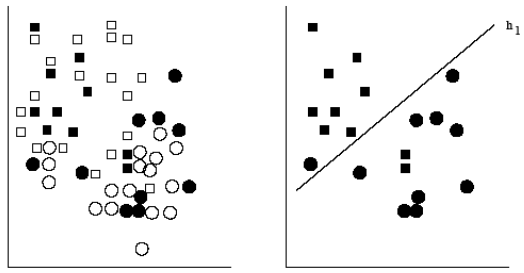
\includegraphics[height=4.5cm]{images/theorie/boosting1}
		\end{center}
		\rule{0pt}{0pt}\hfill{\fontsize{.15cm}{0cm}\selectfont\textit{Source : Cours Machine Learning, Haytham \textsc{Elghazel}}}
	}%
	\only<2>{
		\paraTitle{Deuxième modèle}
		\begin{center}
			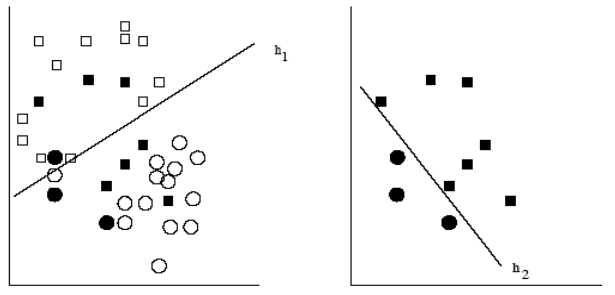
\includegraphics[height=4.5cm]{images/theorie/boosting2}
		\end{center}
		\rule{0pt}{0pt}\hfill{\fontsize{.15cm}{0cm}\selectfont\textit{Source : Cours Machine Learning, Haytham \textsc{Elghazel}}}
	}%
	\only<3>{
		\paraTitle{Troisième modèle}
		\begin{center}
			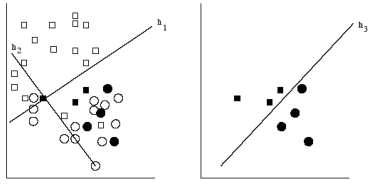
\includegraphics[height=4.5cm]{images/theorie/boosting3}
		\end{center}
		\rule{0pt}{0pt}\hfill{\fontsize{.15cm}{0cm}\selectfont\textit{Source : Cours Machine Learning, Haytham \textsc{Elghazel}}}
	}%
	\only<4>{
		\paraTitle{Vote majoritaire}
		\begin{center}
			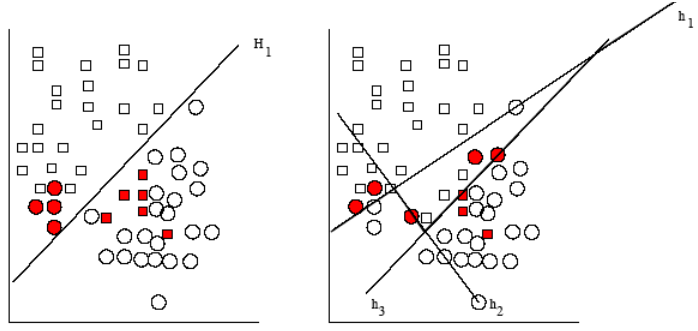
\includegraphics[height=4.5cm]{images/theorie/boosting4}
		\end{center}
		\rule{0pt}{0pt}\hfill{\fontsize{.15cm}{0cm}\selectfont\textit{Source : Cours Machine Learning, Haytham \textsc{Elghazel}}}
	}
\end{frame}

\begin{frame}
	\frametitle{Gradient Boosting et arbres}
	\only<1>{
		\paraTitle{Un arbre simple (CART)}
		\begin{center}
			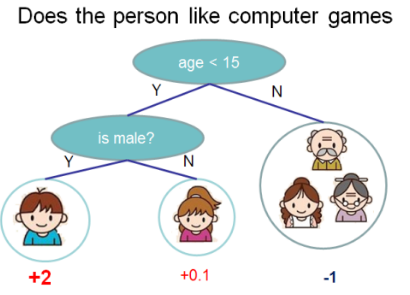
\includegraphics[height=4.5cm]{images/theorie/arbres1}
		\end{center}
		\rule{0pt}{0pt}\hfill{\fontsize{.15cm}{0cm}\selectfont\textit{Source : \texttt{https://xgboost.readthedocs.io/en/latest/model.html}}}
	}%
	\only<2>{
		\paraTitle{Plusieurs arbres vallent mieux qu'un}
		\begin{center}
			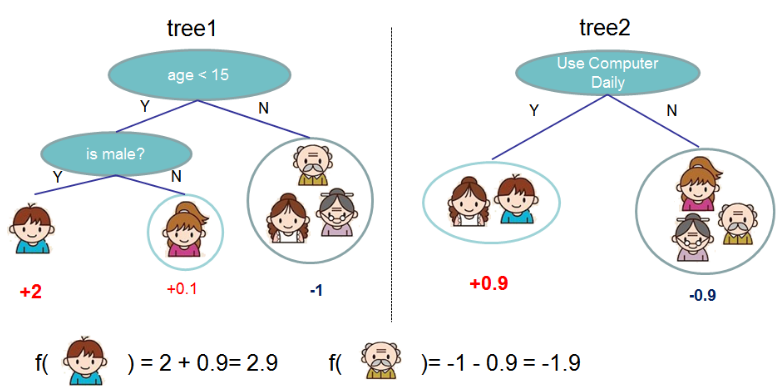
\includegraphics[height=4.5cm]{images/theorie/arbres2}

			Additive training (Boosting)
		\end{center}
		\rule{0pt}{0pt}\hfill{\fontsize{.15cm}{0cm}\selectfont\textit{Source : \texttt{https://xgboost.readthedocs.io/en/latest/model.html}}}
	}%
	\only<3-7>{
		\paraTitle{Choix de l'arbre à ajouter}
	}%
	\only<3>{
		\begin{itemize}
			\itemperso{Fonction objectif}$\textnormal{obj}(\Theta)=\mathcal{L}(\Theta)+\Omega(\Theta)$
		\end{itemize}
		\begin{center}
			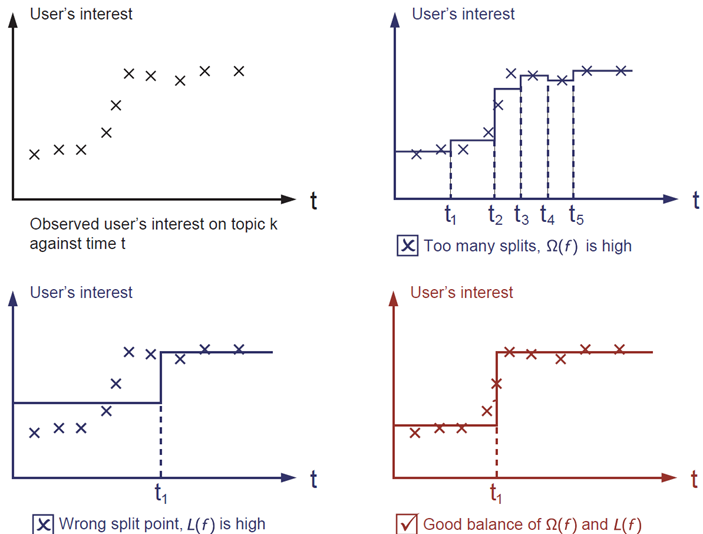
\includegraphics[width=.6\textwidth]{images/theorie/reg}
		\end{center}
		\rule{0pt}{0pt}\hfill{\fontsize{.15cm}{0cm}\selectfont\textit{Source : \texttt{https://xgboost.readthedocs.io/en/latest/model.html}}}
	}%
	\only<4>{
		\begin{itemize}
			\itemperso{Fonction de perte}$\displaystyle{\mathcal{L}(t) = \sum_{i=1}^n\left[g_if_t(x_i)+\frac{1}{2}h_if_t^2(x_i)\right]}$
			\itemperso{Complexité}$\displaystyle{\Omega(t)=\gamma T + \frac{1}{2}\lambda\sum_{j=1}^{T}\omega_j^2}$
		\end{itemize}
		\begin{center}
			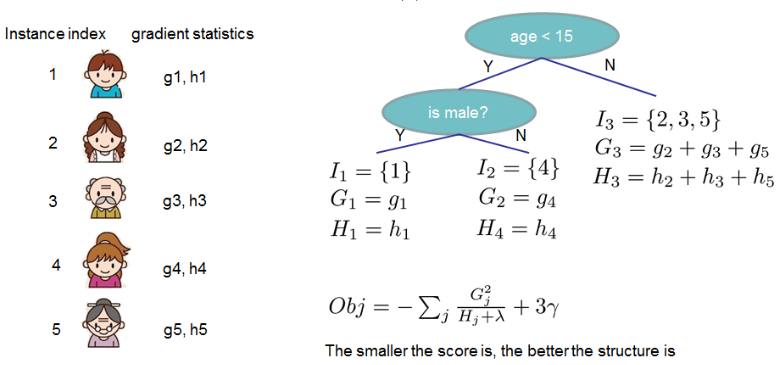
\includegraphics[width=.6\textwidth]{images/theorie/arbres3}
		\end{center}
		\rule{0pt}{0pt}\hfill{\fontsize{.15cm}{0cm}\selectfont\textit{Source : \texttt{https://xgboost.readthedocs.io/en/latest/model.html}}}
	}%
	\only<5-6>{
		\begin{itemize}
			\itemperso{}\'Enumérer toutes les structures d'arbres possibles.
			\itemperso{}Calculer l'objectif pour chaque structure.
			\itemperso{}Trouver l'optimal et optimiser les feuilles.
		\end{itemize}
	}%
	\only<6>{
		\vspace*{.5cm}
		\textbf{En pratique, construction des arbres au coup par coup.}
	}
	\only<7>{
		\begin{itemize}
			\itemperso{Le gain}$\displaystyle{\frac{1}{2}\left[\frac{G_L^2}{H_L+\lambda} + \frac{G_R^2}{H_R+\lambda}-\frac{(G_L+G_R)^2}{H_L+H_R+\lambda}\right]-\gamma}$
		\end{itemize}
		\begin{center}
			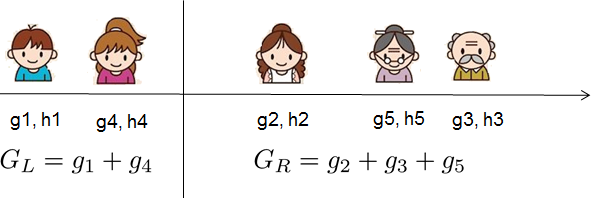
\includegraphics[width=.6\textwidth]{images/theorie/arbres4}

			On ne s'arrête pas si Gain$<$0.
		\end{center}
		\rule{0pt}{0pt}\hfill{\fontsize{.15cm}{0cm}\selectfont\textit{Source : \texttt{https://xgboost.readthedocs.io/en/latest/model.html}}}
	}
\end{frame}

\begin{frame}
	\frametitle{Plus qu'une méthode de Boosting}
	\begin{itemize}
		\itemperso{}Prise en compte de la régularisation.
		\itemperso{}Calcul en parallèle.
		\itemperso{}Support de Hadoop.
		\itemperso{}Possibilité d'adaptation des fonctions objectifs.
		\itemperso{}Prise en charge des valeurs manquantes.
		\itemperso{}Version améliorée de l'élagage
		\itemperso{}Cross-validation native
	\end{itemize}
\end{frame}

\begin{frame}
	\frametitle{Importance des variables}
	\begin{itemize}
		\itemperso{}Entraîner les arbres.\vspace*{.2cm}
		\itemperso{}Pour chaque chaque variable :
		\begin{itemize}
			\subitemperso{}Compter le nombre de fois où elle est sélectionnée.
			\subitemperso{}Pondérer par la diminution d'erreur engendrée.
			\subitemperso{}Moyenner sur les arbres.
		\end{itemize}
	\end{itemize}
\end{frame}

\begin{frame}
	\frametitle{Performances}
	La rapidité est le but initial de XGBoost :
	\begin{itemize}
		\itemperso{Mémoire}Pas de mémoire dynamique.
		\itemperso{Cache}\'Eviter de surcharger la mémoire.
		\itemperso{Amélioration modèle}Voir précédemment.
		\itemperso{Conception}Parallélisation en arrière plan.
		\itemperso{Données externalisées}Si mémoire insuffisante.
	\end{itemize}
	\only<1>{
		\rule{0pt}{0pt}\hfill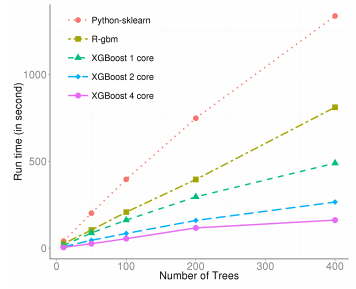
\includegraphics[height=3.5cm]{images/theorie/speed}\hfill\rule{0pt}{0pt}

		\rule{0pt}{0pt}\hfill{\fontsize{.15cm}{0cm}\selectfont\textit{Source : \texttt{http://www.jmlr.org/proceedings/papers/v42/chen14.pdf}}}
	}%
	\only<2>{
		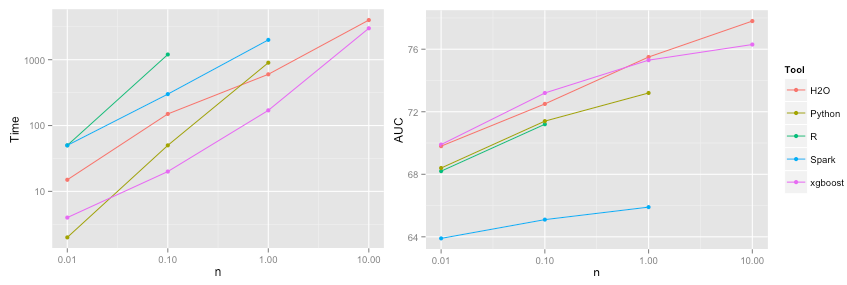
\includegraphics[height=3.2cm]{images/theorie/perf_rf1}

		\rule{0pt}{0pt}\hfill{\fontsize{.15cm}{0cm}\selectfont\textit{Source : \texttt{http://datascience.la/benchmarking-random-forest-implementations/} [2015]}}	
	}
\end{frame}

% Implémentations de XGBoost
\section{Mise en \oe uvre}
\begin{frame}
	\frametitle{Bref historique}
	\only<1>{
		\paraTitle{Sur le boosting}
		\begin{itemize}
			\itemperso{1989}Boosting (R. Schapire)
			\itemperso{1996}AdaBoost (Y. Freund et R. Schapire)
			\itemperso{1999}GBM (L. Breiman puis J. Friedman)
			\itemperso{2014}XGBoost (T. Chen)
		\end{itemize}
	}
	\only<2->{
		\paraTitle{Pour XGBoost}
		\begin{itemize}
	}
		\only<2->{
			\itemperso{Mars 2014}Premières release
			\itemperso{Mai 2014}Python
		}
		\only<3->{
			\itemperso{Septembre 2014}Parallélisation, R
			\itemperso{Mai 2015}YARN, gestion HDFS, SKLearn wrapper
		}
		\only<4->{
			\itemperso{Janvier 2016}API JAVA, amélioration R et Python
			\itemperso{Juillet 2016}C++11, JVM Package (JAVA et Scala)
		}
	\only<2->{
		\end{itemize}\vspace*{\fill}
	}
	\only<2>{
		\rule{0pt}{0pt}\hfill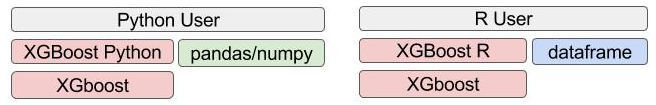
\includegraphics[width=.8\textwidth]{images/implementation/v1}\hfill\rule{0pt}{0pt}
	}
	\only<3>{
		\rule{0pt}{0pt}\hfill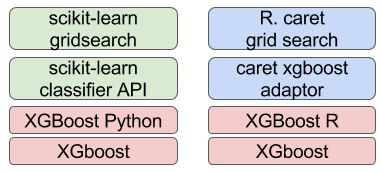
\includegraphics[width=.6\textwidth]{images/implementation/v2}\hfill\rule{0pt}{0pt}
	}
	\only<4>{
		\rule{0pt}{0pt}\hfill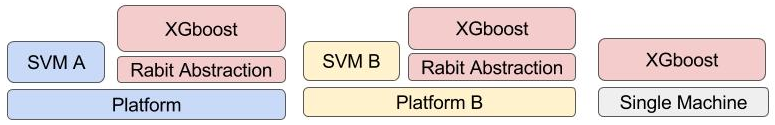
\includegraphics[width=.8\textwidth]{images/implementation/v3}\hfill\rule{0pt}{0pt}
	}
	\only<2->{
		\vspace*{\fill}\rule{0pt}{0pt}

		\rule{0pt}{0pt}\hfill{\fontsize{.15cm}{0cm}\selectfont{\textit{Source : \texttt{http://homes.cs.washington.edu/\~tqchen/2016/03/10/story-and-lessons-behind-the-evolution-of-xgboost.html}}}}
	}
\end{frame}

\begin{frame}
	\frametitle{Des syntaxes proches}
	%bst = xgb.train(param, dtrain, num_round, watchlist)
	%bst <- xgboost(data = train$data, label = train$label, max_depth = 2, eta = 1, nrounds = 2,
    %           nthread = 2, objective = "binary:logistic")
    %bst = xgboost(dtrain, num_round, param = param, watchlist = watchlist,
    %          metrics = ["logloss", "error"])
\end{frame}

\begin{frame}
	\frametitle{Trois familles de paramètres}
	\paraTitle{Paramètres génériques}
	
	Pour définir par exemple quelle méthode Boosting sera utilisée.
	
	\paraTitle{Paramètres liés au Boosting}
	
	Pour paramétrer le booster choisi.
	
	\paraTitle{Paramètres liés à l'apprentissage}
	
	Dépend de la tâche d'apprentissage (classification,...).
\end{frame}

\begin{frame}
	\frametitle{Paramètres génériques}
	\begin{itemize}
		\itemperso{\texttt{Booster}}Linéaire ou arbre.\vspace*{.2cm}
		\itemperso{\texttt{Silent}}Affichage de messages.\vspace*{.2cm}
		\itemperso{\texttt{Nthread}}Par défaut le maximum possible.\vspace*{.2cm}
	\end{itemize}
\end{frame}

\begin{frame}
	\frametitle{Paramètres liés au Boosting}
	\textit{Pour celui sur les arbres. Douze paramètres utiles...}\vspace*{.2cm}

	\begin{itemize}
		\itemperso{\texttt{eta}}Contrôle du niveau d'apprentissage.
		\itemperso{\texttt{Min\_child\_weight}}Pour contrôler l'over/under-fitting
		\itemperso{\texttt{Max\_depth}}Pour contrôler l'over-fitting.
		\itemperso{\texttt{Subsample}}Fraction d'observations à utiliser pour les arbres.
		\itemperso{\texttt{Lambda}}Pour de la régularisation.
		\itemperso{...}
	\end{itemize}
\end{frame}

\begin{frame}
	\frametitle{Paramètres liés à l'apprentissage}
	\begin{itemize}
		\itemperso{\texttt{Objective}}Fonction objectif à minimiser (linéaire, softmax, softprob,...).
		\itemperso{\texttt{Eval\_metric}}Métrique d'évaluation (erreur MSE, MAE, LogLoss, AUC,...).
		\itemperso{\texttt{Seed}}Pour l'aléatoire.
	\end{itemize}
\end{frame}

\begin{frame}
	\frametitle{Quelques bonnes pratique}
	\begin{itemize}
		\itemperso{1.}Fixer un niveau d'apprentissage élevé
		\itemperso{2.}Trouver le nombre optimal d'arbres
		\itemperso{3.}Gérer les paramètres des arbres.
		\itemperso{4.}Gérer les paramètres de régularisation.
		\itemperso{5.}Réduire le niveau d'apprentissage.
	\end{itemize}
\end{frame}

% Applications de XGBoost
\section{Applications}
\iffalse
\begin{frame}
	\frametitle{Médical : exemple de la grippe}
	\begin{center}
		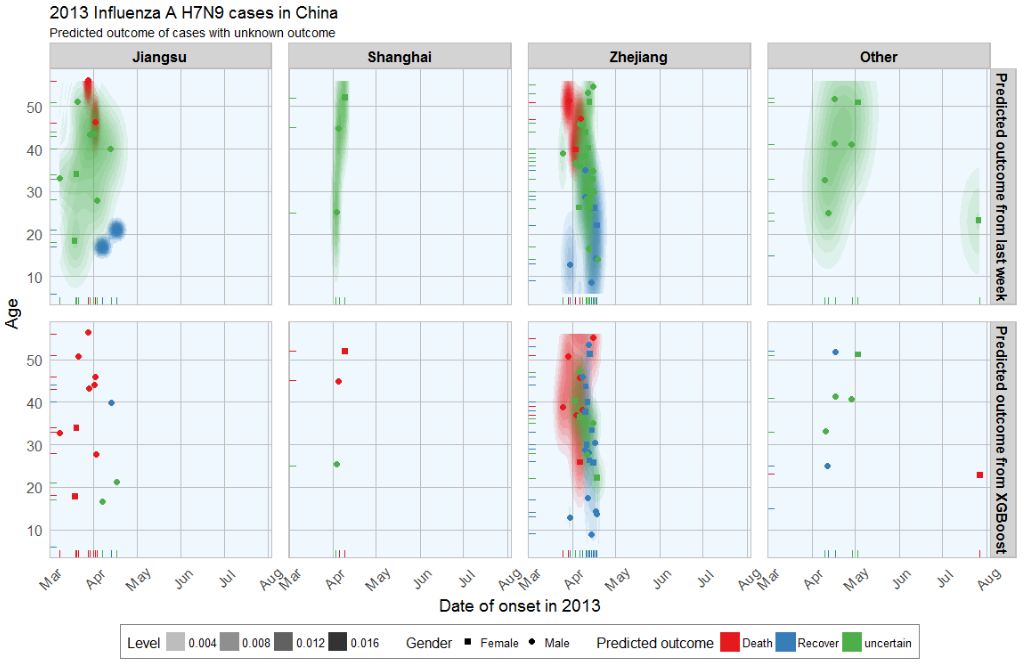
\includegraphics[width=.8\textwidth]{images/utilisation/flue}
	\end{center}
	\rule{0pt}{0pt}\hfill{\fontsize{.15cm}{0cm}\selectfont{\textit{Source : \texttt{https://shiring.github.io/machine\_learning/2016/12/02/flu\_outcome\_ML\_2\_post}}}}
\end{frame}
\fi

\begin{frame}
	\frametitle{Challenges Kaggle}
	\onslide<1->{
		\begin{center}
			\textit{En 2015 sur Kaggle, 17 solutions gagnantes sur 29 utilisaient XGBoost.}
		\end{center}
	}%
	\onslide<2>{
		\begin{itemize}
			\itemperso{1\up{er}}Knowledge Discovery and Data Mining Cup 2016 (V. Sandulescu).
			\itemperso{1\up{er} et 3\up{ème}}CERN LHCb experiment Flavour of Physics competition 2015 (V. Mironov).
			\itemperso{1\up{er}}Caterpillar Tube Pricing competition (M. Filho).
			\itemperso{2\up{ème}}Airbnb New User Bookings (K. Kuroyanagi).
			\itemperso{2\up{ème}}Allstate Claims Severity (A. Noskov).
			\itemperso{10\%}Higgs Boson Competition (T. Chen).
			\itemperso{...}
		\end{itemize}
	}
\end{frame}

\begin{frame}
	\frametitle{Un exemple concret}
	\begin{center}
		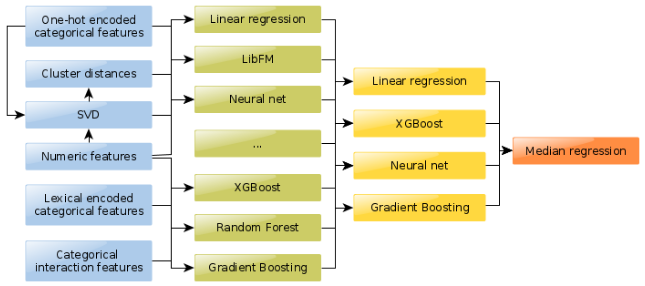
\includegraphics[width=.9\textwidth]{images/utilisation/pipeline}
	\end{center}
	\rule{0pt}{0pt}\hfill{\fontsize{.15cm}{0cm}\selectfont{\textit{Source : \texttt{http://blog.kaggle.com/2017/02/27/allstate-claims-severity-competition-2nd-place-winners-interview-alexey-noskov/}}}}
\end{frame}

\begin{frame}
	\frametitle{En entreprise}
	\textit{Des données difficiles à obtenir...}\vspace*{.2cm}
	\begin{itemize}
		\itemperso{}ODPS Cloud Service (Alibaba)\vspace*{.2cm}
		\itemperso{}Tencent (QQ)\vspace*{.2cm}
		\itemperso{}AutoHome\vspace*{.2cm}
		\itemperso{}AXA, Expedia, Amazon,...\vspace*{.2cm}
	\end{itemize}
\end{frame}

% Conclusion du rapport
\section{Conclusion}
\nnsection{Conclusion}

%%% Local Variables:
%%% mode: latex
%%% TeX-master: "../../Rapport_dreches"
%%% End:


\end{document}